\documentclass[a4paper,12pt,english]{article}
\usepackage[nottoc,numbib]{tocbibind}

\usepackage[utf8x]{inputenc}

\usepackage[english]{babel}
\usepackage{amsmath}
\usepackage{amssymb}
\usepackage{listings}
\usepackage{booktabs}
\usepackage{graphicx}
\usepackage{makeidx}
\usepackage{titlesec}
\usepackage{fancyhdr}
\usepackage{wrapfig}
\usepackage{fancyvrb}
\usepackage{pbox}
\usepackage{hyperref}
\usepackage{mathtools}
\usepackage{amsmath}
\usepackage{multicol}
\usepackage{tocloft}%
\usepackage[refpage]{nomencl}
\usepackage{etoolbox}
\usepackage{longtable}
\usepackage{hyperref}
\usepackage{color}
\usepackage{xcolor}
\apptocmd{\sloppy}{\hbadness 10000\relax}{}{}
\usepackage{nomencl}
\pagenumbering{roman}

\makenomenclature


\graphicspath{ {/} }
\pagestyle{fancy}
\definecolor{lightgray}{rgb}{.9,.9,.9}
\definecolor{darkgray}{rgb}{.4,.4,.4}
\definecolor{purple}{rgb}{0.65, 0.12, 0.82}
\lstdefinelanguage{javascript}{
  keywords={break, case, catch, continue, debugger, default, delete, do, else, false, finally, for, function, if, in, instanceof, new, null, return, switch, this, throw, true, try, typeof, var, void, while, with},
  morecomment=[l]{//},
  morecomment=[s]{/*}{*/},
  morestring=[b]',
  morestring=[b]",
  ndkeywords={class, export, boolean, throw, implements, import, this},
  keywordstyle=\color{blue}\bfseries,
  ndkeywordstyle=\color{darkgray}\bfseries,
  identifierstyle=\color{black},
  commentstyle=\color{purple}\ttfamily,
  stringstyle=\color{red}\ttfamily,
  sensitive=true
}

\lstset{
   language=JavaScript,
   backgroundcolor=\color{lightgray},
   extendedchars=true,
   basicstyle=\footnotesize\ttfamily,
   showstringspaces=false,
   showspaces=false,
   numbers=left,
   numberstyle=\footnotesize,
   numbersep=9pt,
   tabsize=2,
   breaklines=true,
   showtabs=false,
   captionpos=b
}

\setcounter{secnumdepth}{4}
\setcounter{tocdepth}{4}


%Setting link borders to none
\hypersetup{pdfborder = {0 0 0}}

\fancyhead[C]{}
\fancyhead[L]{}
\fancyhead[R]{\footnotesize{
Sebastian O. Jensen}}


\begin{document}

\begin{titlepage}

\newcommand{\HRule}{\rule{\linewidth}{0.4mm}}
\center
\small{ \emph{Forfatter:}\\
14.06-79 Sebastian O. Jensen \textsc{GJX653}
} \\[2cm]

\textsc{\LARGE KEA}\\[0.5cm]
\textsc{\large}\\[1.5cm]
\textsc{\huge Nodejs}\\
\HRule \\[0.7cm]
{\bfseries Keywords: Node.js, MongoDB, Express, AngularJS, Docker,
RESTfull, Web service}\\[0.4cm]
\HRule
\\[1.5cm] \textsc{\Large \textsc{\today}}\\[0.5cm]

\end{titlepage}
\tableofcontents

\pagenumbering{arabic}

\clearpage
\subsection{Abbreviations}
\renewcommand{\nomname}{}
\renewcommand{\pagedeclaration}[1]{}

\printnomenclature[3cm]
\clearpage
\section{Introduction}
\subsection{Abstract}
Forecasts say that in 2020 there will be 25 billion devices connected to the
Internet. In 2014 there was around 3.7 billion devices\cite{Gartner}.
This put a big demand on common technologies such as relational
databases, sessions bassed communication, etc. This project
is a part of a larger project that investigates how to deal with
these challenges. The project does this by designing a system that
meets these challenges. The system consists of multiple devices which connect
in a local network and send information to a backend system over the internet.
This is a realistic example of how to deal with the future of
IoT\nomenclature{IoT}{Internet of Things}. The application consist of the
following items
\begin{enumerate}
  \item Battery powered devices that communicate via the ZigBee protocol.
  \item ZigBee/Internet gateway.
  \item Backend developed using Node.js and the database MongoDB
  \item Frontend developed in AngularJS.
\end{enumerate}

As this project is about the backend system (3) this report does only
describe the other parts when this is needed to describe the functionality of
the backend.

\subsection{Overview of this report}
In section 1.3 is the background for the system described. Section 2 will give a
theoretical background on the technologies which will be used
to implement the backend. Section 3 will give a technical description on the
implementation. Section 4 contains the conclusion.

\subsection{Background}
Internet of Things is a term that describes networks of physical devices that
are connected to the Internet. This can be anything like sensors, wearables,
fridges, heating systems, light balls and what ever could be imagined to
connect to the Internet.
As mentioned there is a high growth in the number of these devices.
This project is about solving a common problem in leisure harbors. 
In leisure harbors there are a limited number of moorings. Therefore it will be
an advantage if a sailer can see if there are free moorings/berths in a harbor
before arriving. 

\section{Theoretical background}
\subsection{REST}
REST stand for Representational State Transfer. Its a method for designing
networked applications.
\nomenclature{REST}{Representational State Transfer}
One of the most important constraints in REST is that it is stateless. Stateless
means that every request should contain all information to process the event. In this
way session state is stored on the client which avoid the need for sessions.
When using sessions the server will need to hold information
about all the devices sessions while communicating. This makes it more difficoult to scale the system
as request can not so easely be load ballanced between multiple servers. Another
thing is that it put a higer demand on the server if it needs store session
state for each connected object. Whith rest load balancing is easy it does not
matter to which server the request is sent as the request holds all information to process the event.

\subsection{Database system}
\subsubsection{Relational database database}
Relational Database Management Systems (RDBMS)\nomenclature{RDBMS}{Relational
Database Management Systems} store data in tables. Access or modification to
data is done using Structured Query Language (SQL)
\nomenclature{SQL}{Structured Query Language}. It was developed in the 1970s and
has been the de facto standard for many years. 

\subsubsection{NoSQL database}
Doing the 2000s an alternative to the RDBMS start to become popular.
The NoSQL Databases. NoSQL stands for ``not only SQL''. \nomenclature{NoSQL}{not
only SQL}There are different ways the NoSQL can store data. But what they have
in common is that they use an object orientated approach. Some of the NoSQL
databases are graph databases that are good at handling graph data. This could
be data in a social network about who is connected to who. Other stores data in
documents or wide-columns \cite{mongo}.
A NoSQL database is often very easy to scale as the developer can just start up
another instance of the DB and the DB will then by it self distribute data among
the DB instances. With SQL DBs it is also possible to divide data on more
servers. But due to the way data is stored this require more work to do. A NoSQL
DB is often many times faster than a SQL DB depending on the job it has to do.
 Three important things to consider when choosing a datastore for a distributed
 system are the following.
 
 \begin{itemize}
   \item Consitency.
   \item Availerbility.
   \item Partition tolerance.
 \end{itemize}
 
 Imagine that a database system is replicated out on to servers, server
 A and B. If data is updated on server A and the same data imediatly being
 retrieved from B before the data has bein replicated then you will get a wrong
 result back. While A and B are not fully syncronised the system is in an
 inconsistant state. Some datastores are higly consitent which means that it is
 not posible to receive ``wrong'' or not updated data. When a system is higly
 consistant it means that all notes se and share the same data.
 Availerbility is about how availerble the system is. A highly availerble
 system garantie that all request will receive a response whitin short time.
 A partition tolerant system garantie that the system will continiu to work even
 when parts of the system is not acceserble do to network link erros.
 
 A theorim called the CAP theorim says that you can only choose to out of the
 tre properties. This makes sense if you think about it. Imagine a system
 should continiue to function when the link between server A and B breaks, at
 the same time be consistent and be able to answer all request imediantly.
 
Each of the three properties can have different importance depending on the
system. Eg. money transfers need high consitency as this is very transaction
critical.

\subsection{Node.js}
Node.js is a javascript runtime environment for developing server side
aplication. It use googles V8 engine. Traditionaly javascript was only being
used as a scripting language on the client side. But Node.js makes javascript
availerble on the serverside as well. What makes node.js speciel is its
architecture. Its single threded which means that it can only do one thing
at a time and has one call stack. Imagine what happens when a resource
requireing task is being executed on the stack. Then the program can't do
anything else. This is called bloking. To avoid bloking the resource requireing
task can be handed over to node.js underlying c++ APIs where the task will be
proccesed outside node.js call stack. When handing over the task a callback
function also need to be provided. When the task is done the callback function
is being put on the callback queue. When there are no tasks on the call
stack, tasks from the callback queue will be processed. This mecanisem is
called the eventloop. And its important to never block the eventloop. By
blooking the event loop is happening if a resource requireing job is
handeled syncroious in the node application. Instead the job should be
handeled asyncrone whit the callback feture. This architecture makes node.js
extreamly fast and able to handle many concurent connections compared to other
serverside platforms. If REST is used in combination with load balance between
more servers the system if very powerfull and easely scalerble. Therefore it is
perfect for applications where there is a high load.

\subsection{Docker}
Docker can in some way be compared to virtual machines but at the same time it
is very much different. A virtual machine simulate a computer which gives the
posibility to run another oporating system on top of the host system. Eg. you
can run a windows oporating system in a virtual machine running on your linux
system. This gives a high overhead as the computer now needs to run to full
oporating systems and the simulation done by the virtual machine program also
take resources. In contrast Docker take an other arcitectual aproach. Docker
is containers which share the kernel and other parts of the oporation system
with the host system. In this way they are a lot more lightweight than virtual
machines. Docker does only run on unix and you can only build unix conainers.
When starting a docker container you need to have an images that defines
the container. Eg. you can start an ubuntu 14.04 container from an ubuntu 14.04
images. There are to ways to obtain an images. One way is to receive it from the
Docker hub or you can build you own images using a Dockerfile. A docker file can
be as simple as the single line ``FROM ubuntu:14.04'' which will build an
ubuntu image. For aditional settings and instalation of programs into the images
aditional lines is needed. Each line in the Dockerfile is actualy a layer.
Layers is also shared between different images if they fit for each other. But it will be out
of the scope of this report to go into all the details about how docker
handles layers. A docker container is only suposed to run one application. If
a server needs to run more applications then you are suposed to start one
container for each application. One of the main advantages of using docker is
that the containers are easy to move around so time is safed on instaling servers and
dealing with compability problems because of different enviroments.
When starting more docker containers on one system they can easely be connected
by linking them to each other. It is also posible to mount host folders inside
the containers.
\clearpage

\section{Design of the backend}
This section covers the design of the backend system. To give a better
understanding of the role and responsibilities of the backend an brief
description of the hole architecture is described in section -----------
below. Then ---------------------------

\subsection{Architecture}
An acrhitecture drawing of the hole system can be viewed in fig. \ref{uml}
below. 

\begin{figure}[h]
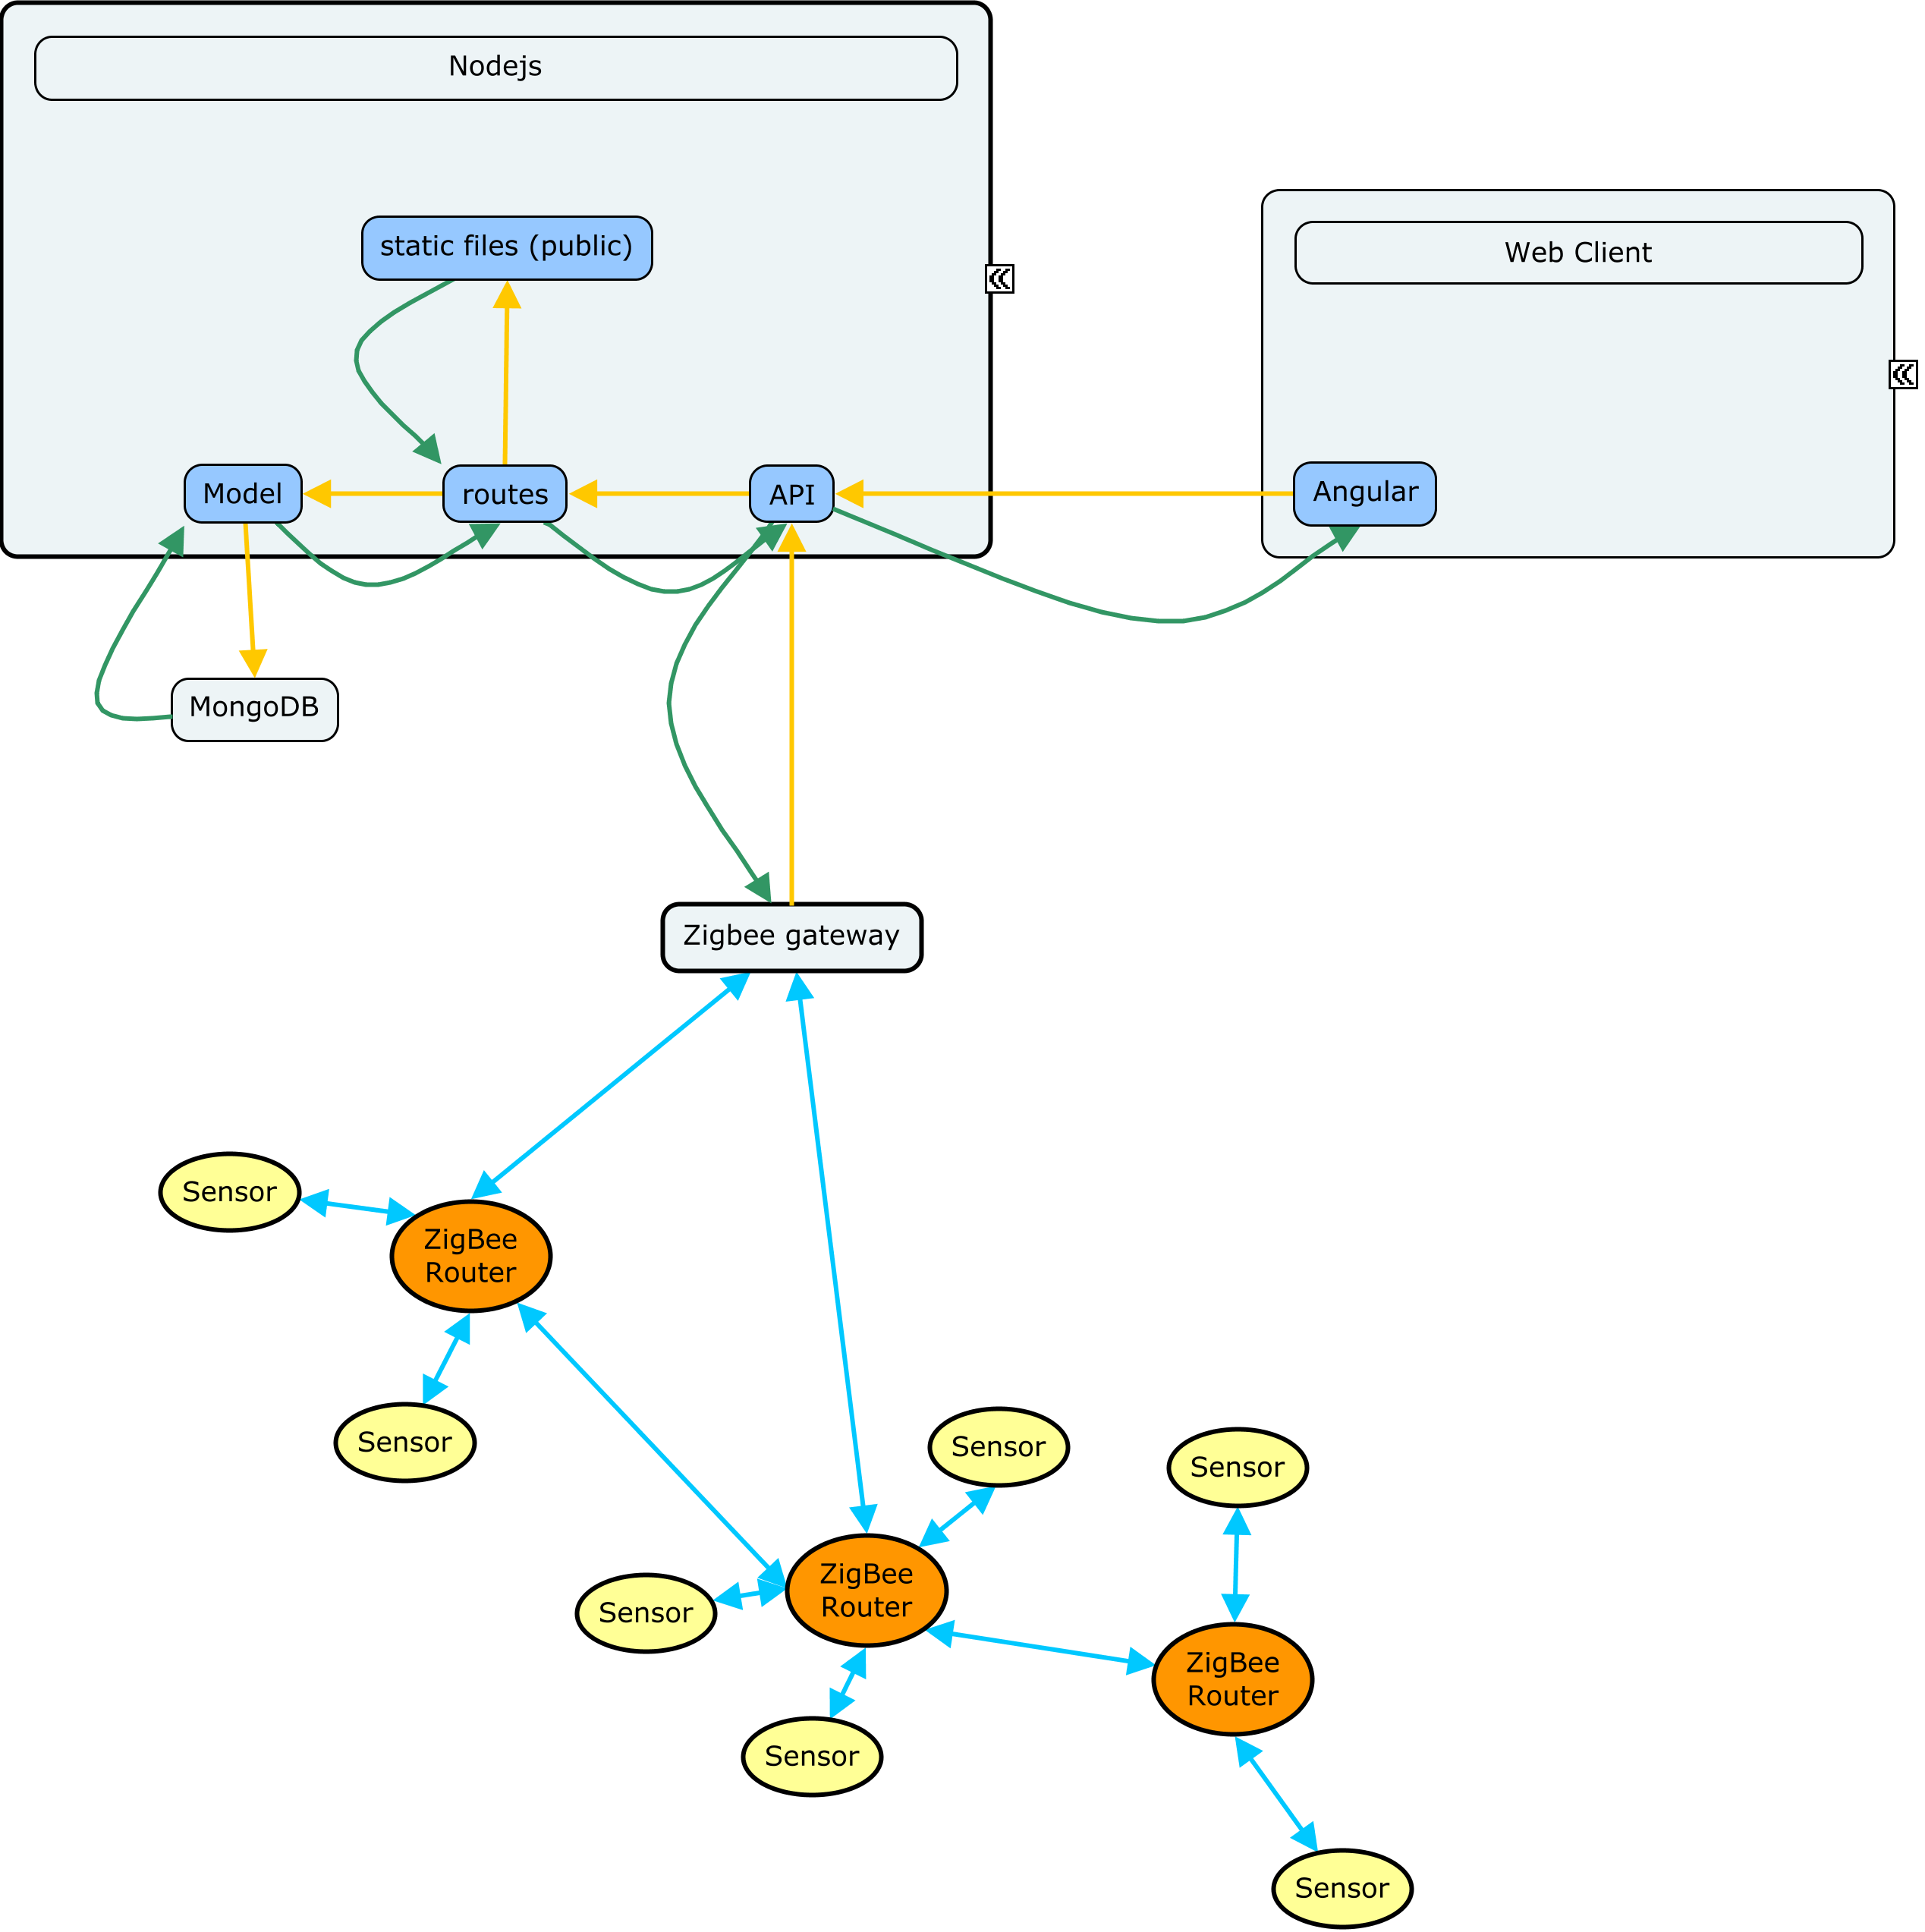
\includegraphics[scale=0.15]{img/architecture.png}
\caption{Architecture}
\label{uml}
\end{figure}

Here follow a short description of each component
\begin{itemize}
  \item Each sensor coorspond to one berth in the harbour. They comunicate via
  the ZigBee routers to the ZigBee gateway. At regular interval they check if
  there is a boat at the berth or not. When there are any changes they send a
  message about the change to the zigbee gateway
  \item The ZigBee gateway translate the messages from the sensors to a JSON
  message which holds information about the state (ocupied / not ocupied) of the
  sensor and the unic id of the sensor. It sends the json message as a PUT
  messages to the backend. As the message contains both the id and the new state
  of the sensor it does not break the RESTfull constraints.
  \item The Node.js application is the heart of the system. The application is
  responsible exposing webservices and handle the datastore which in this
  system is a Mongo database. The application expose RESTfull webservices that
  are being consumed by the ZigBee gateway and the frontend.
  \item The Mongo database store all the data. The date is user information and
  the information about the state of each berth.
  \item The webclient runs the frontend application which is developed in
  AngularJS. Angular is responsible for render and present the information
  received from the backend.
\end{itemize} 


\subsection{Requirements of the backend}
To show how the backend work some requirements has been defined and implemented.
In a full production ready system aditional functianlities is required. These
aditional requirements will be discused in the sections below and in the
conclution. But for now we will do with the following recurements.

\begin{itemize}
	\item Expose a RESTfull api which can receive information about the state of
	each berth in the port and store the information.
	\item Expose RESTfull api's which make data accesible to the frontend.
	\item Be able to handle authentication.
	\item Let admins update users and see all users.
\end{itemize}


\subsubsection{MongoDB}
As descibed in the theoretical section a NoSQL database is often many times
faster than a relational database\cite{mongotest}. Mongo is an object related
database which fits our data as each sensor can be seen as an object. Mongo can be used as a
higly consitant and partition tolerant database. It priorities these proberties
on the cost of availerbility. When mongo is distributed on more servers the
consitancy is garantied if you use looking. You can look on different levels
(document, collection or database level). Locking on collection or
database level can be usefull when dealing with transactions \cite{mongoManual}
Therefore Mongo is a good choise to use as a database.


\subsubsection{Nodejs}
Node.sj comes with the NPM package
manager which can be used to easely install libraries and extensions. For this
application the Express web framework is used. Express is
unopinionated about how you are building stuff. This means that you Express
does not set any rules about how you build you application. This makes it very
flexible and a good choice for building web APIs. Express feature midleware
which give the posibilities to devide different task to different middle ware.
Eg. all request to restricted services can be passed by a midleware which check
for authentication. Each middleware can be passed the request and response
objects, which the midleware can access and modify. When the midleware is done
it passes on the request and response object to the next middleware until a
response is send to the requesting client.
Things will be more clear when describing the source code in section
------------------------------------------------

\section{Implementation}
\subsection{Folder structure}
The project is structured in folders. A list of folders and files in the root
folder is shown in fig \ref{rootFolder}. The Dockerfile and runSystem.sh
files are related to setting up and running the system. The folder mongoVol
is a folder where the Mongo database store its data. README.ml is a file used by
GIT\footnote{GIT is a version control system. It is outside the scope of this
report to explain details abput git} to describe the project. port.iml is a
projectfile for and IDE which is not relevant. The folder named port
contains the Node.js and Express application. The content of this folder wil be
described in the following section

\begin{center}

\begin{figure}[h]
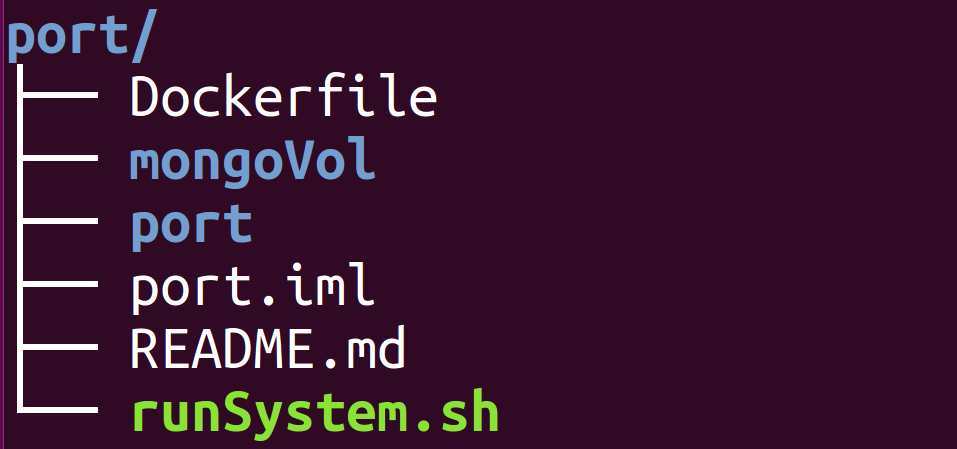
\includegraphics[scale=0.2]{img/rootFolder.png}
\caption{Rootfolder of the project. Blue is folders, white is files, green is
executerble files.}
\label{rootFolder}
\end{figure}
\end{center}


\subsection{Nodejs and Express}
The project have been build over the MVC pattern by deviding the data model, controler, and the views.

\subsubsection{Folder structure}
In fig \ref{express} the folder structure of the Node, Express and AngularJS is
shown.
The sub folder public contains the frontend AngularJS application. The other
parts is related to the backend application which will be described in details
in the next sections.

\begin{center}
\begin{figure}[h]
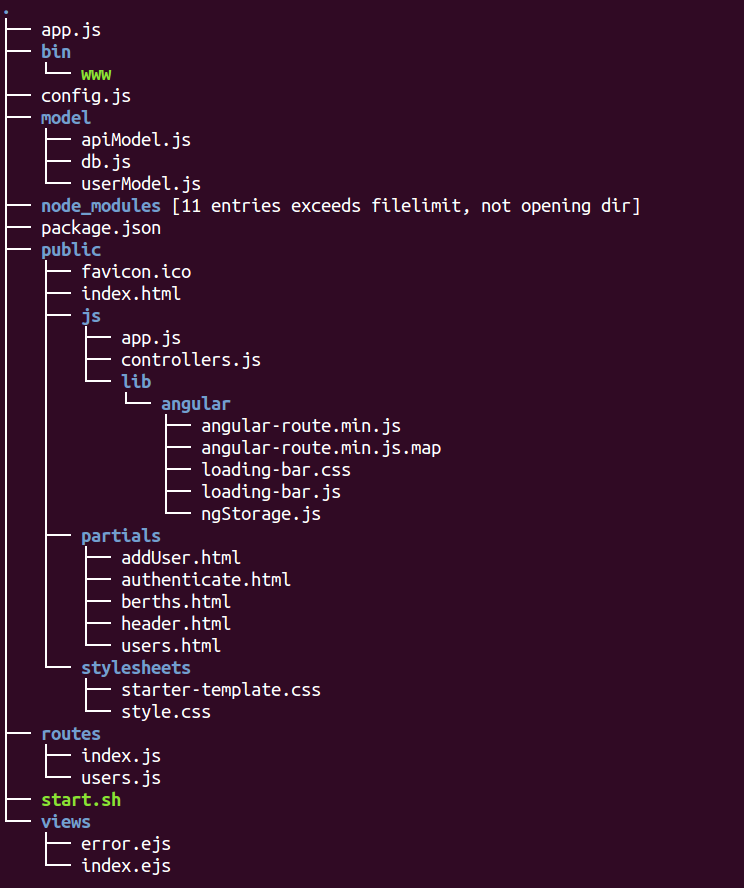
\includegraphics[scale=0.45]{img/express.png}
\caption{Folder structure of Nodejs, Express and AngularJS. Blue is folders,
white is files, green is executerble files.}
\label{express}
\end{figure}
\end{center}

\subsubsection{NPM, package.json and modules}
As mentioned erlier Node comes with the package manager NPM. NPM packages can be
installed globaly on the system or local to the project. Packages which an
application is dependent on can be specified in the file package json. When you
install a new package to use in you project you can apply the save atribute to
the npm command. This will put the dependecy in to the package.json file. You
can also edit the file manualy. If you enter the command NPM install all
packages in the file will be installed into the folder node\_modules. The
content of package.json is showed here.

\begin{lstlisting}[language=javascript]
{
  "name": "port",
  "version": "1.0.0",
  "private": true,
  "scripts": {
    "start": "node ./bin/www"
  },
  "dependencies": {
    "body-parser": "~1.13.2",
    "cookie-parser": "~1.3.5",
    "debug": "~2.2.0",
    "ejs": "~2.3.3",
    "express": "~4.13.1",
    "jsonwebtoken": "^5.4.1",
    "mongo": "^0.1.0",
    "mongodb": "^2.0.48",
    "morgan": "~1.6.1",
    "serve-favicon": "~2.3.0"
  }
}
\end{lstlisting}

This application are using 10 modules. Here follow a brief description of each
module.
\begin{itemize}
\item body-parser: Used for parsing the content from and to the body of a html
messages. In this project it is used for parsing Json data
\item cookie-parser: Used forhandling cookies
\item debug: Used by express to write debug messages
\item ejs: For handling embedded Javascript templates on the frontend. (Not
used by this project. but it comes with express. Could actually be removed)
\item express: The web framework
\item jsonwebtoken: Used for authentication using tokens
\item mongo: a wrapper for the mongoDB driver. (Is not used in this project)
\item mongodb: The native driver for Mongo
\item morgan: Used for logging
\item serve-favicon: Used for seting the favicon
\end{itemize}

\subsubsection{aap.js}
In the file app.js the initialication is defined. A big part of
this file is generated by express it self. Here an object named app is created
which is the nerve of the application. Here folow a description of what has
been changed for this project. In the top of the file, needed modules are
imported with the requier statement. 2 lines has been added

\begin{lstlisting}[language=javascript]
var config = require('./config')
var db = require('./model/db');
\end{lstlisting}s

The first file config is a file that has been made for holding speciel
configuration parameeters. For now the only configuration parameeter that is
handeled here is a secret used to create and validate tokens. But more stuff
shuld be moved here. Eg. database url and login would be good to place in the
config file.
\\
\\
The line
\begin{lstlisting}[language=javascript]
app.set('superSecret', config.secret); 
\end{lstlisting}
Sets a variable in the app object to hold the value of the secret.
\\\\
The connection to the database is establised
\begin{lstlisting}[language=javascript] 
db.connect('mongodb://db/zigbee', function(err) {
  if (err) {
    console.log('Unable to connect to Mongo.')
    process.exit(1)
  }
  else {
    console.log('Connected to DB')
  }
})
\end{lstlisting}
As node js is asyncron it is important to mention
 \\
The line
\begin{lstlisting}[language=javascript]
console.log("running in " + app.get('env') + " mode"); 
\end{lstlisting}
Prints the environment mode. This will be explained later.

The line
\begin{lstlisting}[language=javascript]
app.use(express.static(__dirname + 'public'));
\end{lstlisting}
set the public folder to the path for static content. 


\subsubsection{Model}
The model handles access to the mongo database. The model makes an abstraction to the application about how access to an underlying datastore is done. In this way the application does not need to consentrate on how data is accessed or which data store is used. In the model folder is one file named db.js. It contains the folowing tree functions
\begin{itemize}
\item connect: this we saw used in the file app.js for connecting to the database.
\item get: To tell the state of the database connection
\item  close: which is used for closing the connection
\end{itemize}
In top of the file the mongo driver is imported with the require statement.
The code can bee viewed in the provide source.
\\
The model folder also contains to  other files $apiModel.js$ og $userModel.js$

These files defines functions which update and get data from the database. The functions are exposed the to the controler which is defined in the routes folder. An example of one of the functions is shown below


\begin{lstlisting}[language=javascript]
exports.updateBerth = function(json, callback) {
  var collection = db.get().collection('berths')
  collection.replaceOne({_id: json._id}, json, {upsert: true}, function(err, response) {
    callback(err, response)
  })
}
\end{lstlisting}
This function updateBerth updates the status of a berth. The {upsert:true} option means that a record shoud be created if it does not exist.
The rest of the functions can be seen in the source files.
\\
The userModel expose the foloving functions.
\begin{itemize}
\item all: Return all the users in the system
\item updateUser: update or create a user
\item getUser: return a user from the database
\end{itemize}

See the source files for the full code.

\subsubsection{Routes and authentication}
The routes control how the application respond to requests. This is done using middleware and pattern maching on the URL and request method.
In the $app.js$ file the following to lines 
\begin{lstlisting}[language=javascript] 
app.use('/', routes);
app.use('/users', users);
\end{lstlisting}
defines that all reguest with the path starting with users should be handeled by the routes deffined in routes/users.js and all other requests should be handeled by routes/index.js

\paragraph{routes/index}
The routes in routes/index.js defines tree routes. Which is the following

\begin{itemize}
\item getAllBerths: GET method for returning all the berth and theis status as json
\item updateBerth: PUT method for updating or creating a berth 
\item root path: This will send the index file of the angular application.
\end{itemize}

Below is the code for the updateBerth path

\begin{lstlisting}[language=javascript] 
router.put('/updateBerth', function(req, res) {
  json = req.body
  apiModel.updateBerth(json, function(err, response) {
    res.json(response);
  })
});
\end{lstlisting}
As we see this midleware will only mach request of the type PUT and the path /updateBerth. first the body of the request is encoded into the variable json. Next the function updateBerth in the apiModel is called with the json object. When the apiModel has done its magic the response from updating the database is send as the response. This is an other example of using callback. And this is one of the wery important places to use the asyncron aproach, because database access is one thing that can slow down the system if we were to wait for every database task to finalize before doing anything else.

\paragraph{routes/users and authentication}
The routes in the routes/users.js files is a litle more complicated. The routes are the following.

\begin{itemize}
\item /authenticate: POST method which Handles authentication
\item /*: ALL methods. This catch every request and is used to check if a user is authenticated
\item /getAllUsers: GET method for returning all the users
\item /updateUser: POST method for adding a user to the system
\end{itemize}

The first method handles the authentication. The code is provided here

\begin{lstlisting}[language=javascript] 
router.post('/authenticate', function(req, res, next) {
  received = req.body;

  userModel.getUser(received, function(err, data) {
    //if there was no data in the db
    if(data === undefined){
      res.json({success: false, message: "Authentication failed"});
    } else{
      if (data.password != received.password){
        res.json({success: false, message: "Authentication failed"});
      } else {
        var token = jwt.sign({userType: 'admin'}, req.app.get('superSecret'));
        res.json({success: true, message: "you are authenticated", token: token})
      }
    }
  })
});
\end{lstlisting}

The function expect to receive a username and a password in the body of the post message. The the coorsponding user is retrieved from the database vie the user model. Then there is no coorsponding user or the password of the user does not mach a response message with text "authentication failed" is send back to the client. If the password mach then a jason web token is created and send back. The token consist of tree parts. A header, payload and signature. In the header we can define the usertype, the payload can contain information about expiration and other detail, the signature is used for checking that the token is valid. The signature is hashed using the secret key which was defined in the config file and set in the app variable seperSecret. The header and payload are not encrypted so the client can read the conten by decoding it with the base 64 algorithm. So its important not to put sentitive stuff here in case a hacker sniff the token. When a user is outhenticated it should send the web token with all the request. In this app this is being done by setting the token in the header.\\

When a user access any other path handeled by the user router, the midleware matching the path /* and regardles of the method will catch everything. This midleware is shown below

\begin{lstlisting}[language=javascript] 
router.all('/*', function(req, res, next) {
  token = req.headers.token;
  console.log(token);
  jwt.verify(token, req.app.get('superSecret'), function(err, decoded) {
    console.log(decoded) // bar
    if (decoded){
      req.authenticated = decoded.userType;
      next();
    } else {
      req.authenticated = null;
      next();
    }
  });
});
\end{lstlisting}
This middleware check if a user is authenticated. It first get the token from the header. Then the token is verified. If the token is valid then a variable named authenticated in the request object is set to the usertype of the user. In this app there are only the usertype admin. If the token is not valid authenticated is set to null. One thing to notice with this middleware is that the callback function get past an object called next. This is used to parse the request on to the next handler. So instead of seting the response the middleware parse on the request which will then be catched by one of the handlers below if any there are any match. Each of the handlers that requiere authentication ofcourse need to be defined below the middleware that checks for authentication. And the handler can then check the authenticated variable and respond depening on the usertype or if no type is set.
Here is an example of the getallusers handler 

\begin{lstlisting}[language=javascript]
  if(req.authenticated == 'admin'){
    userModel.all(function(err, data) {
      console.log(data);
      res.json(data);
    })
  } else {
    res.json({message: 'you do not have access to this page'});
  }
});
\end{lstlisting}
It checks if the user is admin and if so all the users is send back else the messages "you do not have access to this page" is send back.

\subsubsection{Views}
The view folder contains views which is not used in this project as the frontend is handeled by angularJS. Express defaults to use views in a format called JADE . But for testing it was changed to EJS. But as this is not used in the project. Nothing more will be mentioned about this.

\subsubsection{bin/www and start.sh}
Running a node application is as simple as runnng the following command

\begin{lstlisting}[language=javascript] 
node <application>
\end{lstlisting}

But Express provide an executerble file bin/www. In the top of this file the line

\begin{lstlisting}[language=javascript] 
#!/usr/bin/env node
\end{lstlisting}
defines that when running the file it shuld be run with the node application. Instead of using node this project use nodemon instead. The difference between node and nodemon is that nodemon listen for file changes and automaticaly restart when any changes has been made to the source files. This makes development faster as you do not need to manualy restart node to see changes. Therefore the line has been changed to 

\begin{lstlisting}[language=javascript]
#!/usr/bin/env nodemon
\end{lstlisting}

This project use another wrapper $start.sh$ the code in this file is shown below.

\begin{lstlisting}[language=javascript]
#!/bin/bash
cd /www
npm install
#NODE_ENV=production /www/bin/www
/www/bin/www
\end{lstlisting}

When this script is run it first changes directory in to a the folder /www on the system. This is were the application should be placed. Then all dependencies are installed. The next line which is commented out can be used to run the application in production instead of development mode. Running in production mode make some changes to how the application is running. Eg. error messages is not send to the clients and the performance is also better.
Last line run the application.
\clearpage
\subsection{Docker Mongo and runsystem.sh}
The application is run using the docker echo system. This is all handeled by the runSystem.sh script. Downloading the project and running the script on a system that has docker installed will handle all the setup and running the application. The code in the file is showed below.

\begin{lstlisting}[language=javascript]
#!/bin/bash
# uncomment all lines below to make a fresh build of the system

docker stop $(sudo docker ps -a -q)
docker rm $(sudo docker ps -a -q)
rm -rf port/node_modules
docker build -t seeeb/port .
docker pull mongo
docker run --name thisMongo -v ~/port/mongoVol:/data/db -it -d mongo:latest
docker run -d --name nodejs --link thisMongo:db -p 80:80 -it -v ~/port/port:/www seeeb/port
\end{lstlisting}
\begin{itemize}
\item Line 1 define that its a script which should be run by bash
\item Line 4 use the docker ps command to get all running containers and fetch it to the docker stop command. In this way we are shure no other containers are running.
\item Line 5 Remove all the containers. (remeber a container is an instance of a docker image)
\item Line 6 Removes all the modules from the node application to forse a clean install of all the modules.
\item Line 7 builds a docker images named seeeb/port using the Dockerfile. This docker images run the node application and will be explained in the next section.
\item Line 8 pull the latest official mongo image from the docker hub.
\item Line 9 Starts a container of the mongo images, name it thisMongo and maps the host folder ~/port/mongoVol in the container folder /data/db. The -d option demonize the container so it is runing in the background.
\item Line 10 Starts a container using the images seeeb/port and name it nodejs.
  \begin{itemize}
  \item "-d" tell docker to demonize the container. If you want to see the output from node, this should be removed
  \item "--link thisMongo:db" tell that this container should link to the container nammed thisMongo with the alias db. Note that inside the node application when defining the adress to the mongo database we only need to specify "db" as the adress.
  \item "-p 80:80" map the external port 80 of the host system to external port 80 of the the node container
  \item "it" tell that we want to interact with the container and get a shell. in this way the output from the node application is printed to the screen of the host system.
  \item "-v "/port/port:/www" mounts the host folder ~/port/port in the container folder www.
  \end{itemize} 
\end{itemize}

Its important that the project is placed in the home folder of the host system because the shell script expect to find the files here.

\subsubsection{Dockerfile}
The Dockerfile defines the node images. See the code below

\begin{lstlisting}[language=javascript]
FROM ubuntu:14.04

RUN apt-get update && apt-get install -y git python build-essential curl nano wget libkrb5-dev
RUN wget https://nodejs.org/dist/v4.2.1/node-v4.2.1-linux-x64.tar.gz
RUN sudo tar -C /usr/local --strip-components 1 -xzf node*

RUN npm install express -g
RUN npm install express-generator -g
RUN npm install -g nodemon

CMD /www/start.sh
EXPOSE 80:80
\end{lstlisting}

The file is prety much self explanatory. First we specify to start from an uuntu 14.04, rhen all the the dependen packages is installed. Then express and nodemon are installed globaly.
The line $CMD /www/start.sh$ tell that this script should be run when the system has started.
$EXPOSE 80:80$ Make port 80 availerble as a port that can be acced on the container.
\subsubsection{hosting}
The project is hosted on an Amacon EC2 ubuntu server. And a dns record pointing the subdomain port.lapela.dk to it has been seed.

The function can be tested by sending json requests using Chrome Postman to the server or by using the angular frontend application by accessing the the address in a browser. The Angular application provide four functions which is the following
\begin{itemize}
\item Berth: Whitch shows all the berth and their status
\item Users: Which shows all the users if you are outhenticated
\item Add user: Which let you add a user if you are loged in
\item Login: Which authenticated a user
\end{itemize}

A user account with the username "admin" and password "nodeJSkursus" can be
used to test the system. As this server is only running to show the system is
working it is ok to do all kinds of test like adding users, updating berths
status, etc.
Also note that under add user and login some fields is defined in the bottom
that is bind to response message and the stuff you enter in the form. This is to
show what goes on under the hood. This would ofcourse not be there in a
production version of the system.

For testing the updateBerth API a simulater has been developed using Java.
It first choose some random berth id's and then start sending random status
update messages simulating status change. This will result in some new berth
are being added to the system and that those new berth will be updated
randomly. The code of the simulator is handed in together whit this report.
\clearpage
\section{Conclusion}
The aim of the project is to show how a realistic Node.js application can be build also taking into account performance and scalability. It has been showed that Node.js together with MongoDB is a high performance system that easely scale. Looking at the Life in Vista Prints test \cite{mongotest} comparing Mongo with a SQL database it
is clear that the mongo database is faster than a realtional database when
working with object data.
There some things that would need improvement for an system put into
production. This is that passwords should never be stored in the database as
clear tekst. The password strength should also be checked when creating a user
and it should not be allowed to have a week password. Right now you can
actually create a user with no username or password. It is also important that
the access to the side is using ssl. If not, everybody can grap tokens or
passwords flying over the network. Another thing that should also be protected
with JWT is the updateBerth API which at the moment can be mish used by anyone 

All in all this project conclude and show how Node.js, Mongo and Express can be used to build a backend system with high performance and scalerbility
\clearpage

\begin{thebibliography}{9}


\bibitem{Gartner}
  Gartner,
  \emph{ An American information technology research and advisory
  firm}, \url{http://www.gartner.com/newsroom/id/2905717}

\bibitem{zigbeeModel}
ZigBee Pro Specifications,
\emph{ZigBee Alliance},
Full specification can
be downloaded from
bottom of this page
\url{http://www.zigbee.org/zigbee-for-developers/network-specifications/zigbeepro/}

ZigBee Document 053474r20
September 7, 2012 10:19 pm
Sponsored by: ZigBee Alliance
Accepted by ZigBee Alliance

\bibitem{zigbee}
ZigBee Alliance,
\emph{ZigBee Pro, Technical Summary},
\url{http://www.zigbee.org/zigbee-for-developers/network-specifications/zigbeepro/}

\bibitem{802.11ac}
802.11ac A Survival Guide,
\emph{Matthew S. Gast}


\bibitem{mongo}
MongoDB,
\emph{What is NoSQL},
\url{https://www.mongodb.com/nosql-explained}

\bibitem{mongoManual}
MongoDB manual.
\emph{Concyrency},
\url{https://docs.mongodb.org/manual/faq/concurrency/}

\bibitem{mongotest}
MongoDB vs. SQL Server’s XML Data Type
\emph{Lifeinvistaprint.com},
\url{http://lifeinvistaprint.com/techblog/mongodb-vs-sql-servers-xml-data-type/}

\bibitem{flipdot}
AlfaZeta
\emph{flipdots specification},
\url{http://www.flipdots.com/electromagnetic-status-indicators.html#.Vi8uApcy1hE}

\bibitem{CC2530}
Texas Instruments
\emph{CC2530 Specifications},
\url{http://www.ti.com/lit/ds/symlink/cc2530.pdf}

\bibitem{ano79}
Texas Instruments
\emph{Measuring Power Consumption of CC2530 With Z-Stack},
\url{http://www.ti.com/lit/an/swra292/swra292.pdf}

\bibitem{rf04}
Ultrasonic sensor HC-RF04
\emph{ELEC Freaks},
\url{http://www.electroschematics.com/wp-content/uploads/2013/07/HCSR04-datasheet-version-1.pdf}

\bibitem{saft}
Specification of LM 17500 battery
\emph{SAFT batteries},
\url{http://www.saftbatteries.com/force_download/LM17500_datasheet_0515.pdf}

\bibitem{raspberry}
Specification of Raspberry model 2
\emph{Raspberry Pi},
\url{https://www.raspberrypi.org/products/raspberry-pi-2-model-b/}

\bibitem{znp}
ZNP interface specification
\emph{Texas Instruments},
\url{http://e2e.ti.com/cfs-file/__key/communityserver-discussions-components-files/158/3286.CC2530ZNP-Interface-Specification.pdf}


\end{thebibliography}


\clearpage
\textsc{\huge Appendices}
\appendix

\end{document}
